\section*{Modulebeschrijving}
\begin{tabularx}{\textwidth}{|>{\columncolor{lichtGrijs}} p{.26\textwidth}|X|}
	\hline
	\textbf{Module name:} & \modulenaam\\
	\hline
	\textbf{Module code: }& \modulecode\\
	\hline
	\textbf{Study points \newline and hours of effort:} & This module gives \stdPunten{}  ects, in correspondence with \FPeval{\result}{clip(\stdPunten*28)}\result{} hours:
	\begin{itemize}
		\item 3 x 6 hours frontal lecture
		\item 3 x 6 hours practicum
		\item the rest is self-study
	\end{itemize} \\
	\hline
	\textbf{Examination:} & Written examination and practicums (with oral check) \\
	\hline
	\textbf{Course structure:} & Lectures, self-study, and practicums \\
	\hline
	\textbf{Prerequisite knowledge:} & Basic imperative control structures and datatypes, as per INFDEV02-2. \\
	\hline
	\textbf{Learning tools:}  &
		\begin{itemize}
			\item Book: Think Python; author A. B. Downey (\url{http://www.greenteapress.com/thinkpython/})
			\item Book: The Coder’s Apprentice; author Pieter Spronck (\url{http://www.spronck.net/pythonbook/pythonbook.pdf})
			\item Presentations (in pdf): found on N@tschool and on the GitHub repository \url{https://github.com/hogeschool/INFDEV02-2}
			\item Assignments, to be done at home and during practical lectures (pdf): found on N@tschool and on the GitHub repository \url{https://github.com/hogeschool/INFDEV02-2}
		\end{itemize} \\
	\hline
	\textbf{Connected to \newline competences:} &
	\begin{center}
		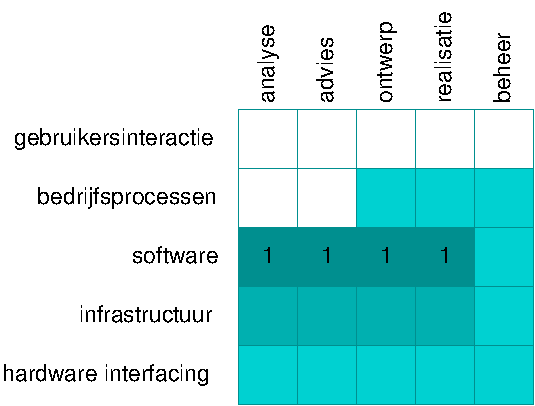
\includegraphics[width=7cm]{comptabel.pdf}
	\end{center}\\
	\hline
	\textbf{Learning objectives:} &
		At the end of the course, the student can:
			\begin{itemize}
               \item \textbf{use} and \textbf{design} recursive functions \texttt{FUNREC}
               \item \textbf{understand} the concept of abstraction through class definition \texttt{CLSABS}
               \item \textbf{use} and \textbf{design} classes without inheritance or interfaces \texttt{CLSDEF}
               \item \textbf{use} recursively defined lists \texttt{LISTS}
               \item \texttt{RECDATA}
               \item \textbf{use} standard predefined collections \texttt{STDDS}
			\end{itemize} \\
		
	\hline
\end{tabularx}
\newpage

\begin{tabularx}{\textwidth}{|>{\columncolor{lichtGrijs}} p{.26\textwidth}|X|}
	\hline
	\textbf{Content:}&
	\begin{itemize}
		\item basic concepts of data structures
		\item list: design of a well-known data structure
		\item functions as abstraction of instructions 
		\item Higher order functions and relation SQL (Python 3)
		\item methods within container of classes (Python 3)
		\item collection libraries: list, tuple, map, set (Python 3)
	\end{itemize} \\
	\hline
	\textbf{Course owners:} & \author\\
	\hline
	\textbf{Date:} & \today \\
	\hline
\end{tabularx}
\newpage
